\section{Resultados}

\subsection{Temperatura y coeficiente de decaimiento}

\subsubsection{Logro de la experimentación}
% - Qué fue lo que se logró con la experimentación 
Con este experimento se pudo determinar que la precisión del k es proporcional a la cantidad de iteraciones, y que a medida que la instancia aumenta en su dimensión, las cantidades de iteraciones son cada vez más relevantes a la hora de encontrar un mejor óptimo.

\begin{figure}[!ht]
    \centering
    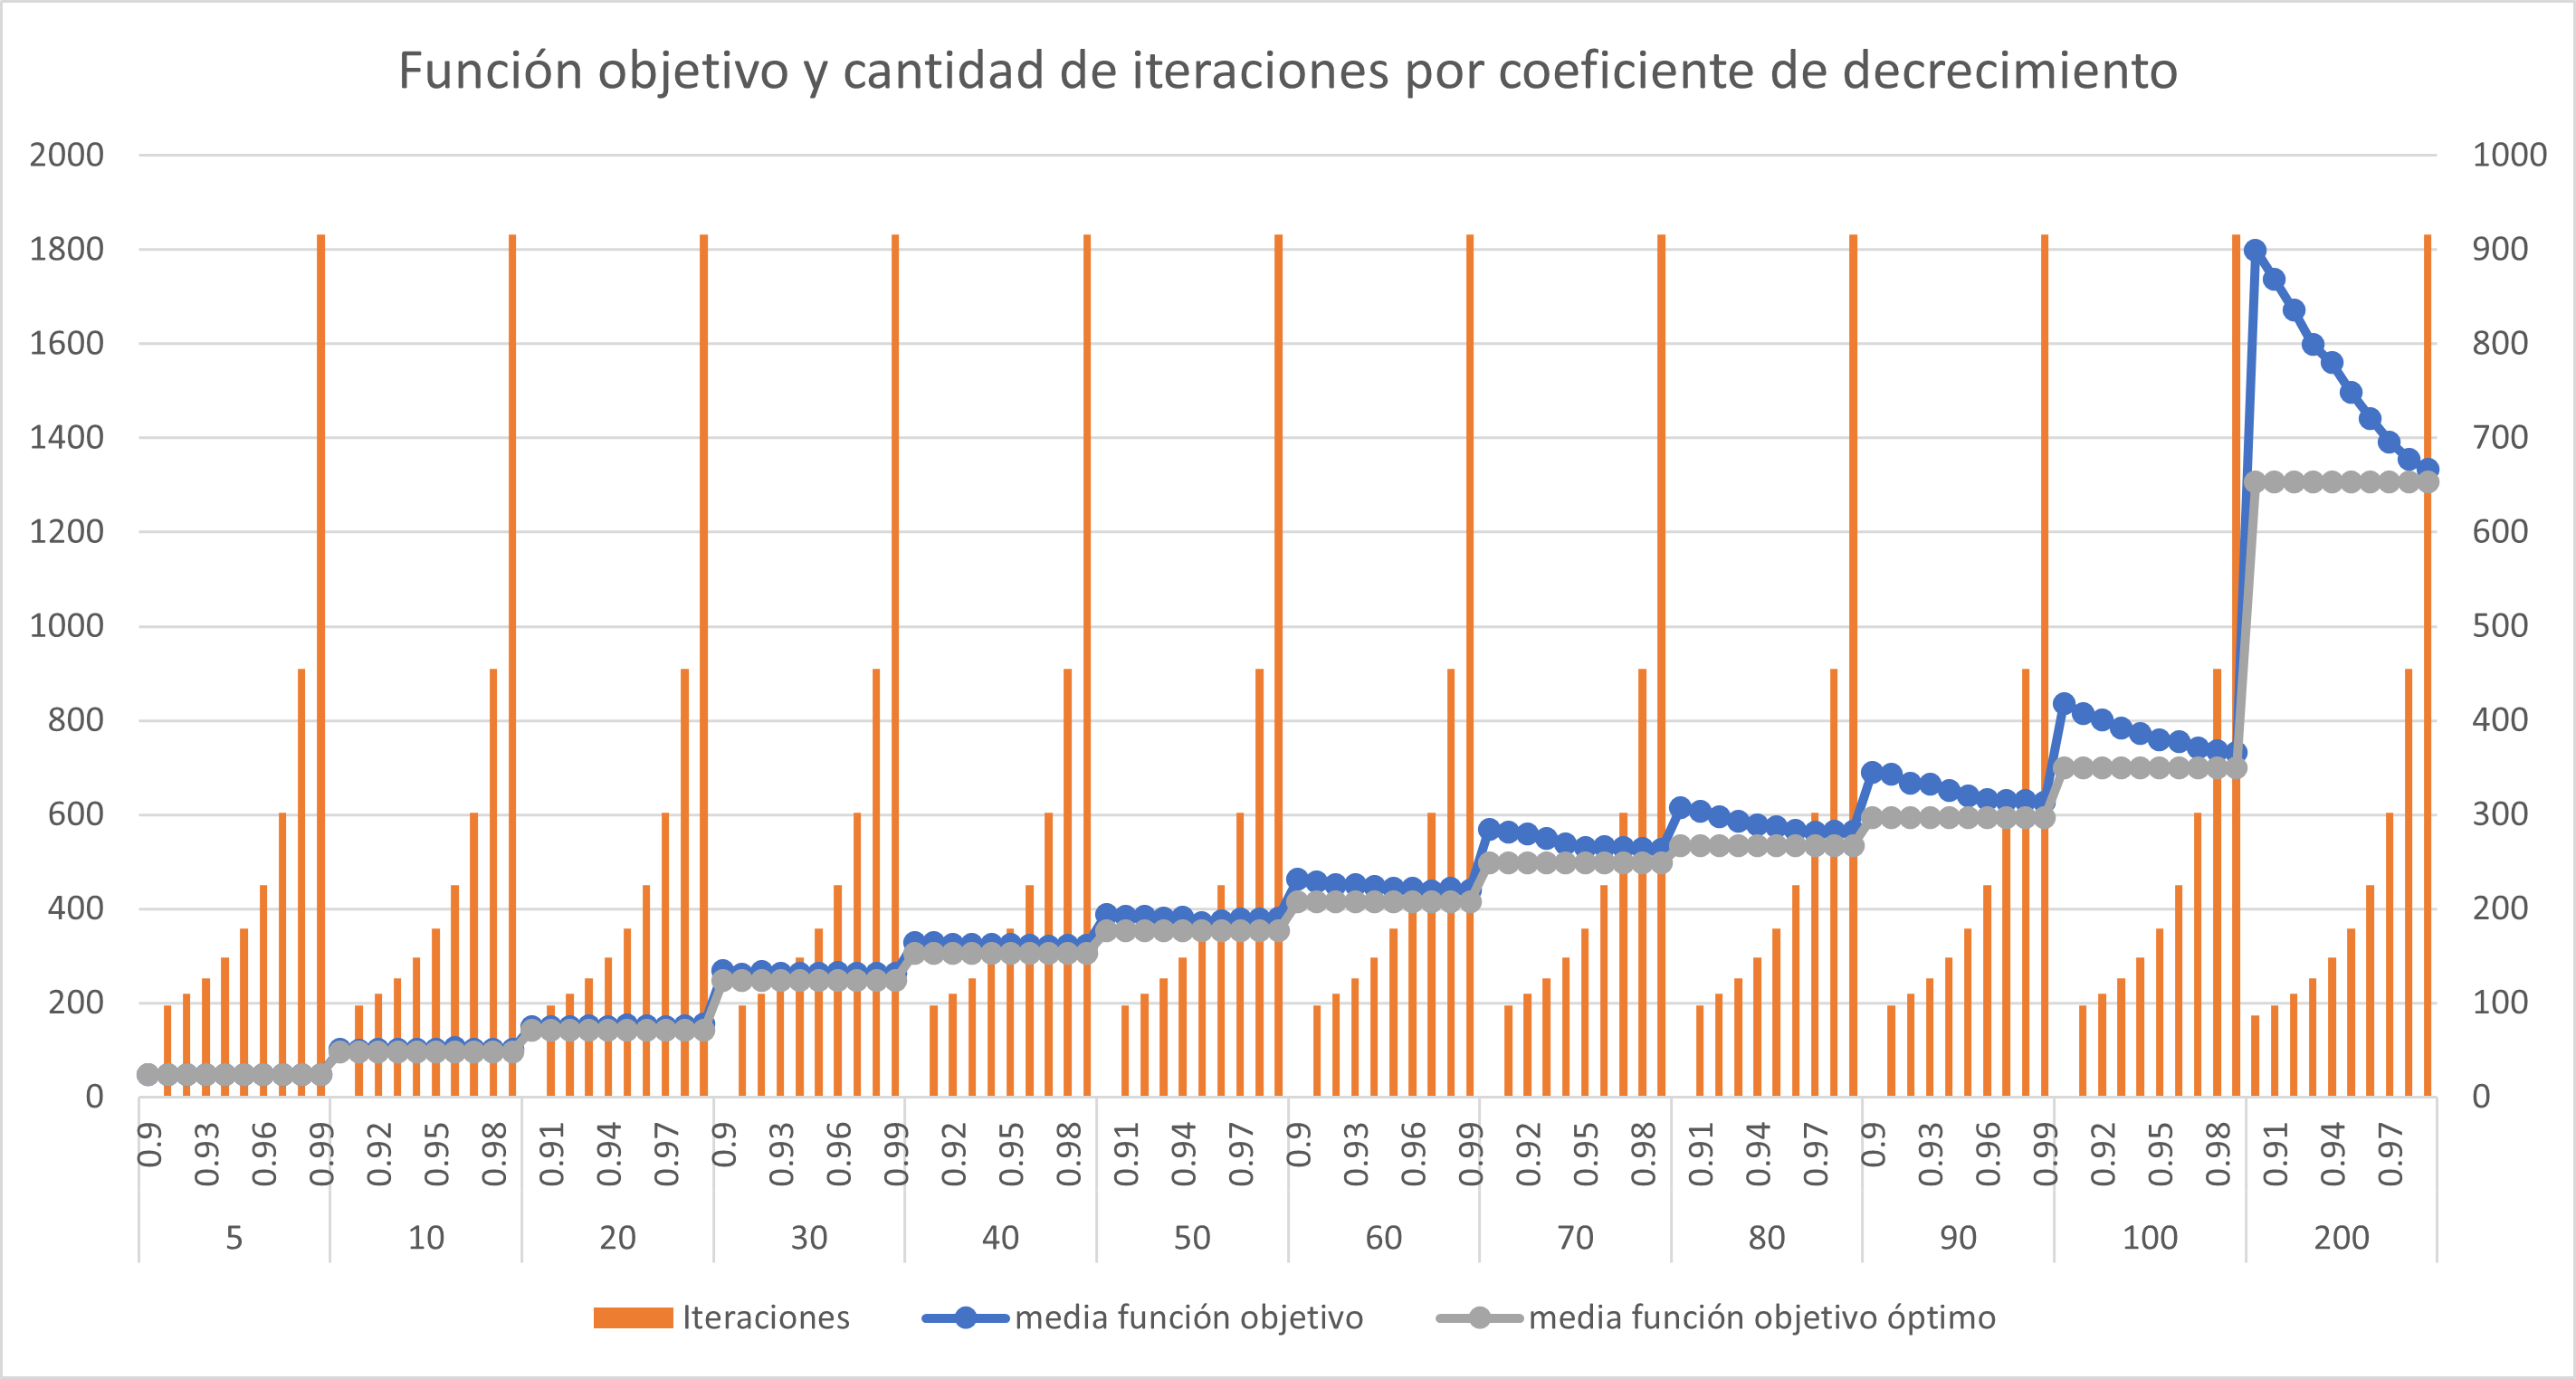
\includegraphics[width=\textwidth]{images/testing/funcion_objetivo_vs_k.png}
    \caption{Función objetivo y cantidad de iteraciones por coeficiente de decrecimiento para todas las instancias.}
    \label{graph:k_all_instances}
\end{figure}

Luego de la experimentación se realizó un gráfico resumen \ref{graph:k_all_instances} que muestra el promedio de los óptimos locales obtenidos para cada instancia con cada coeficiente y para la última instancia de dimensión 200 se puede extraer, como se puede ver en la figura \ref{graph:f_i_por_k_instance_200}, que no existe mayor diferencia entre el coeficiente $0.98$ y $0.99$, con el coeficiente $0.98$ se logra una diferencia entre el óptimo local encontrado por la prueba y el óptimo de referencia de $48.2614$ puntos, con cerca de $455$ iteraciones a diferencia de lo que sucede con el coeficiente $0.99$ que se logra una diferencia de $26.4274$ con casi el doble de iteraciones, siendo casi despreciable en comparación con la diferencia del orden de los $492.4654$ que alcanza el coeficiente $0.90$.

En cambio para una instancia pequeña como la de dimensión 5, ver figura \ref{graph:f_i_por_k_instance_5}, un coeficiente $0.90$ o $0.99$ no afecta en la búsqueda, de hecho siempre se obtiene el óptimo local de referencia, la única gran diferencia es que para un coeficiente de $0.90$, se ejecutan 87 iteraciones y para un coeficiente de $0.99$, se realizan 916 iteraciones.

\begin{figure}[!ht]
    \centering
    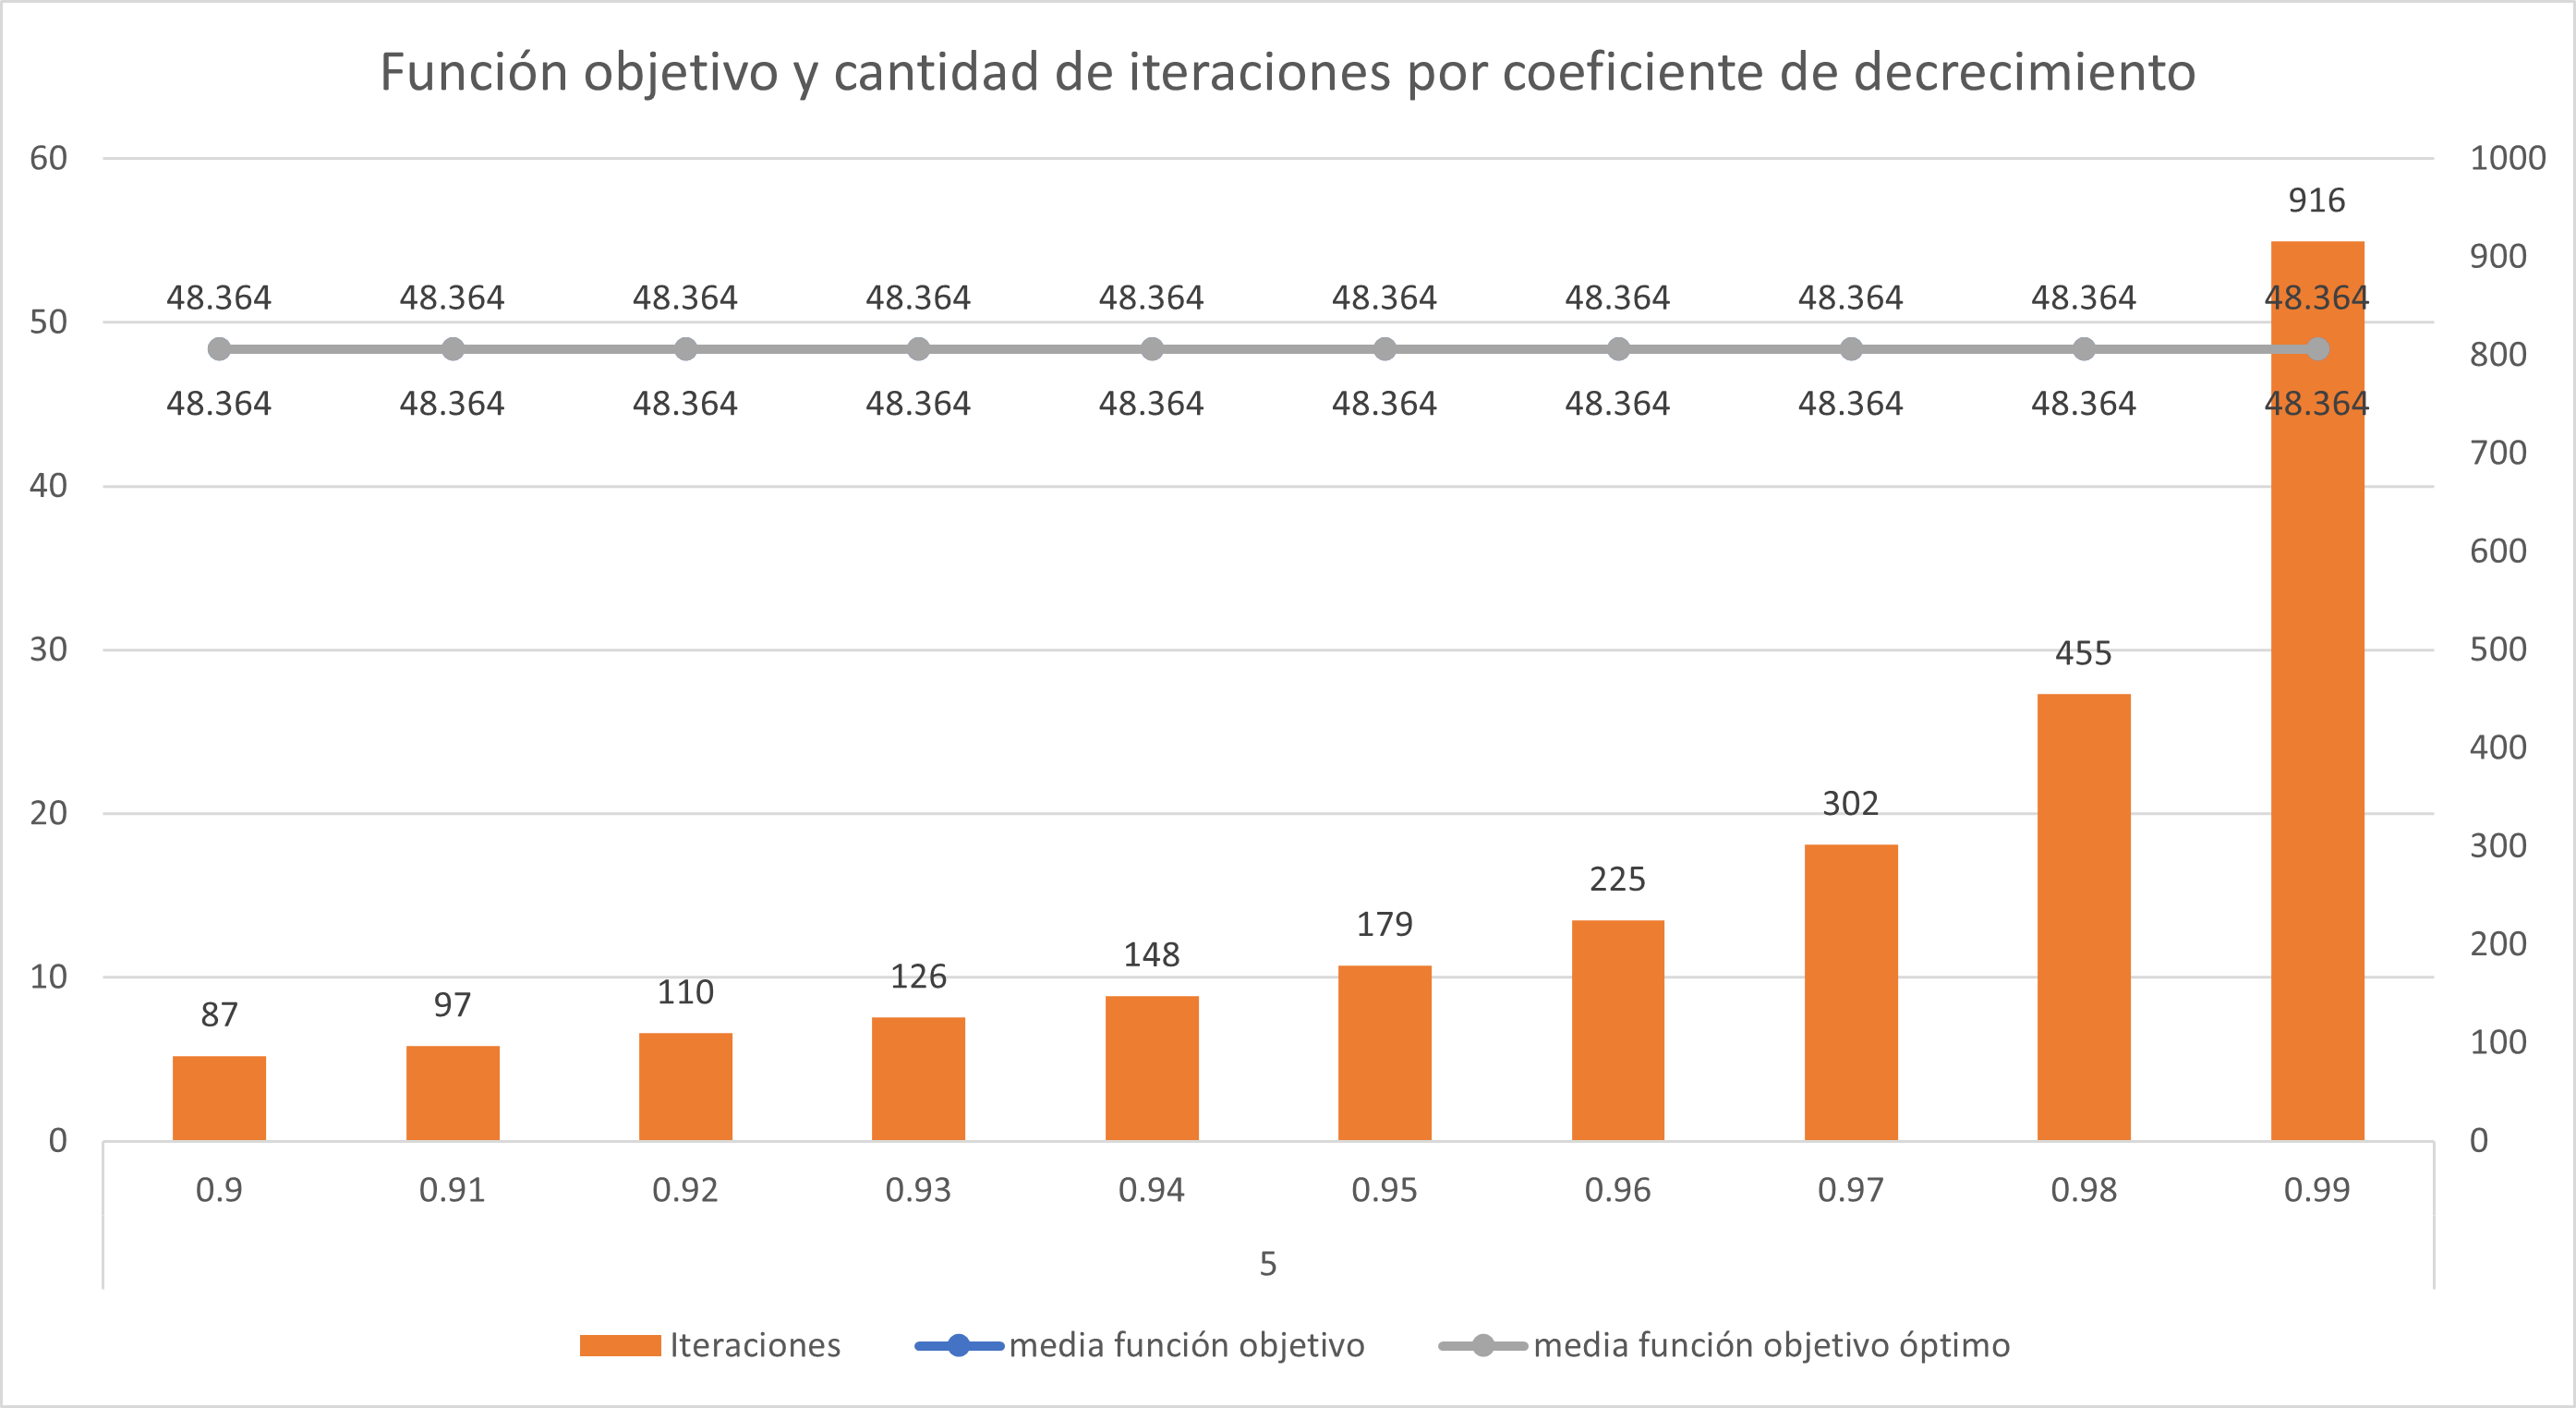
\includegraphics[width=\textwidth]{images/testing/funcion_objetivo_vs_k_5.png}
    \caption{Función objetivo y cantidad de iteraciones por coeficiente de decrecimiento para la instancia de dimensión 5.}
    \label{graph:f_i_por_k_instance_5}
\end{figure}

\begin{figure}[!ht]
    \centering
    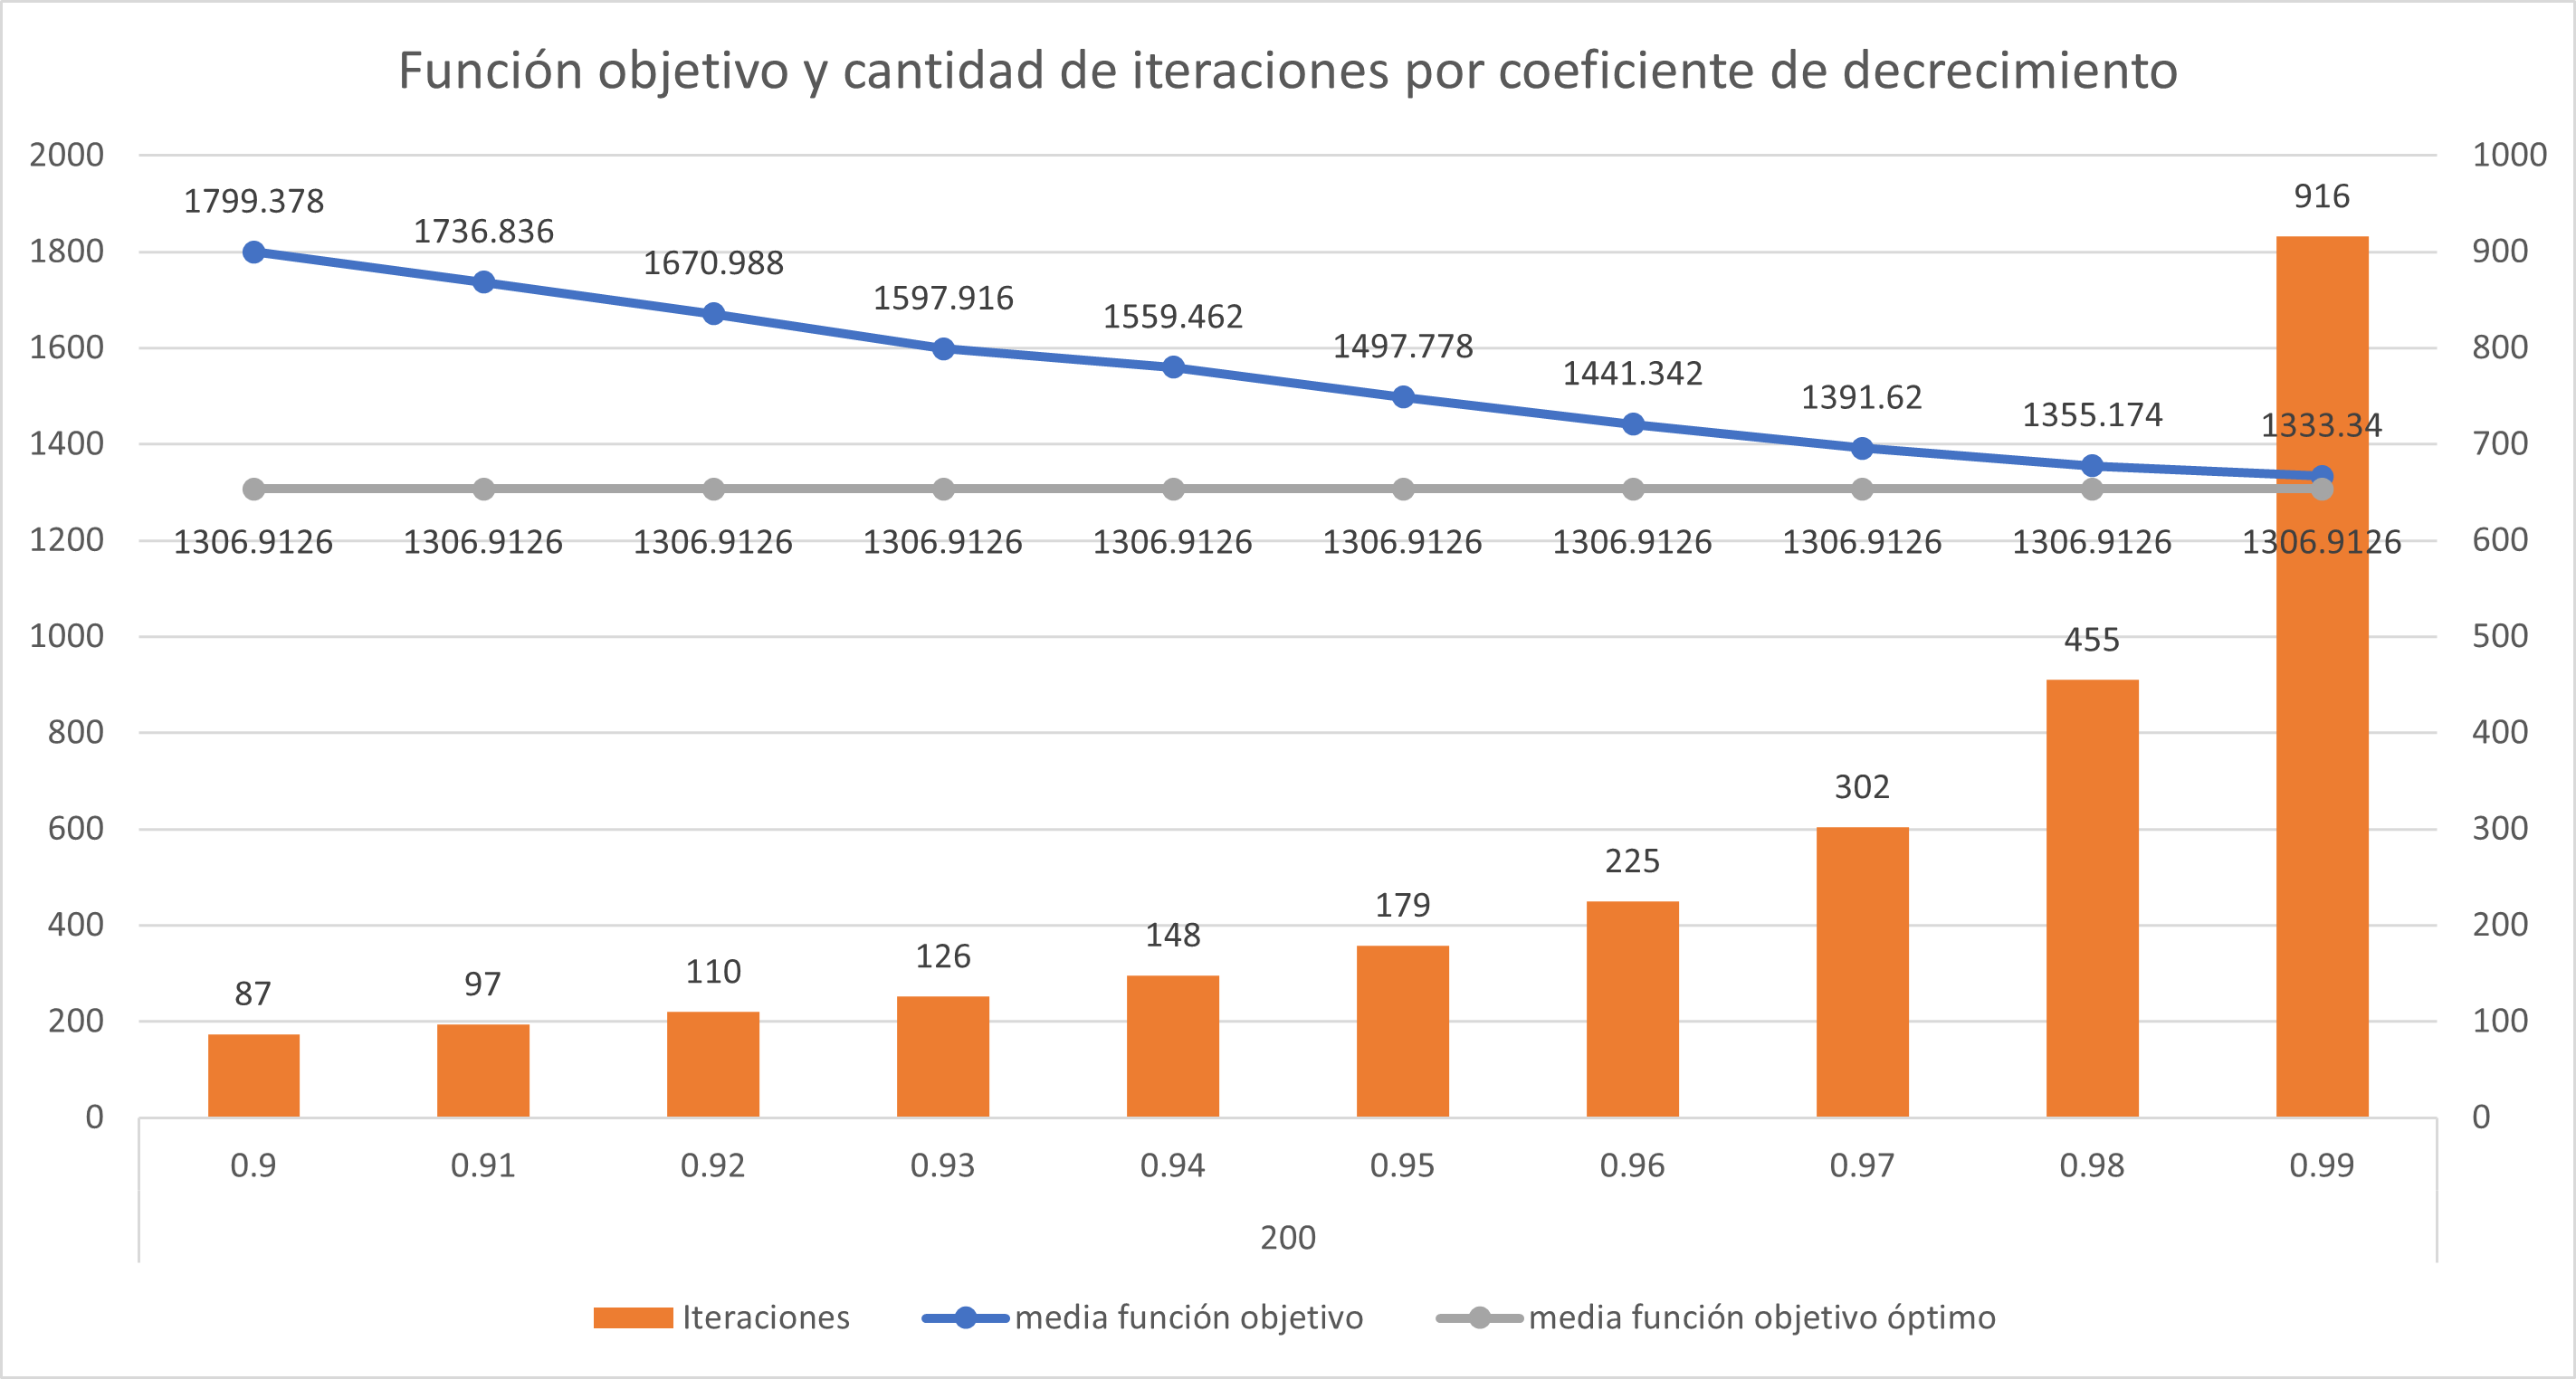
\includegraphics[width=\textwidth]{images/testing/funcion_objetivo_vs_k_200.png}
    \caption{Función objetivo y cantidad de iteraciones por coeficiente de decrecimiento para la instancia de dimensión 200.}
    \label{graph:f_i_por_k_instance_200}
\end{figure}

\subsubsection{Análisis}

Se puede entonces ahora determinar que el coeficiente $0.98$ es un de los mejores coeficientes para encontrar un óptimo aceptable para realizar pruebas, debido a la insignificante diferencia entre los óptimos locales que generan los coeficientes $0.99$ y $0.98$, y la inmensa diferencia entre su cantidad de iteraciones $916$ y $455$, respectivamente

\subsection{Movimiento}

\subsubsection{Logro de la experimentación}

Con la experimentación se logró identificar que el movimiento 2 que corresponde al movimiento completamente iterativo, como se dijo desde un principio no es óptimo para este problema.

Además se identificó una pequeña diferencia entre el movimiento 0 y el 1, como muestran los gráficos \ref{graph:movements_5} y \ref{graph:movements_200}, que representan la media de la función objetivo por movimiento para las instancias $5$ y $200$. Si bien el \textit{movimiento 0} se comporta de mejor manera que el \textit{movimiento 1} en la instancia $200$, no es mucho mejor, solamente una diferencia del orden de los $20$ puntos destructivos. Y se destaca la dificultad que tiene el \textit{movimiento 0} para lograr alcanzar el óptimo de referencia en la instancia de dimensión 5.


\begin{figure}[!ht]
    \centering
    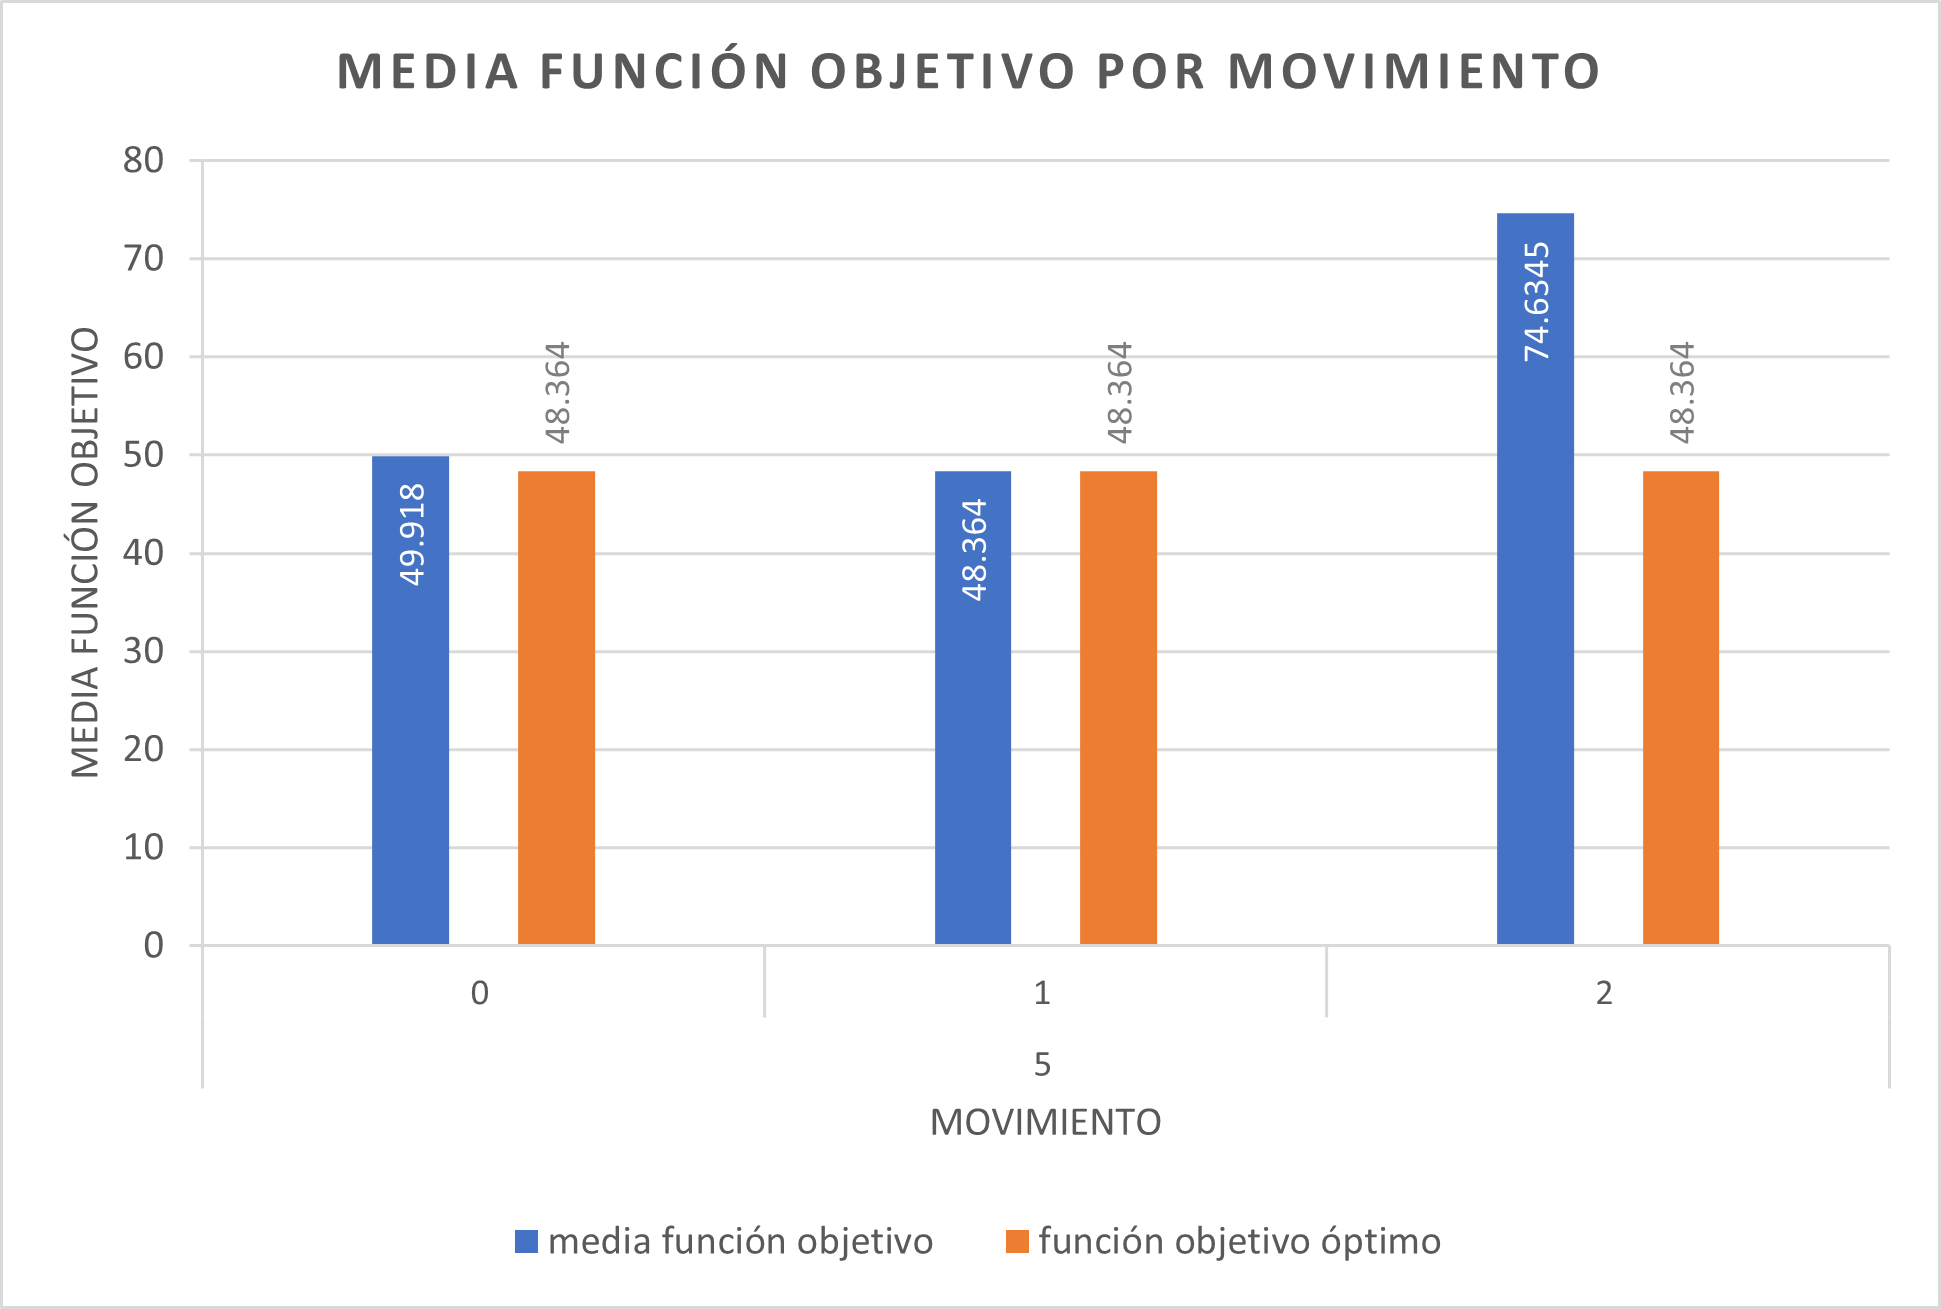
\includegraphics[width=0.8\textwidth]{images/testing/media_por_movimiento_5.png}
    \caption{Media de función objetivo por movimiento para la instancia de dimensión 5.}
    \label{graph:movements_5}
\end{figure}

\begin{figure}[!ht]
    \centering
    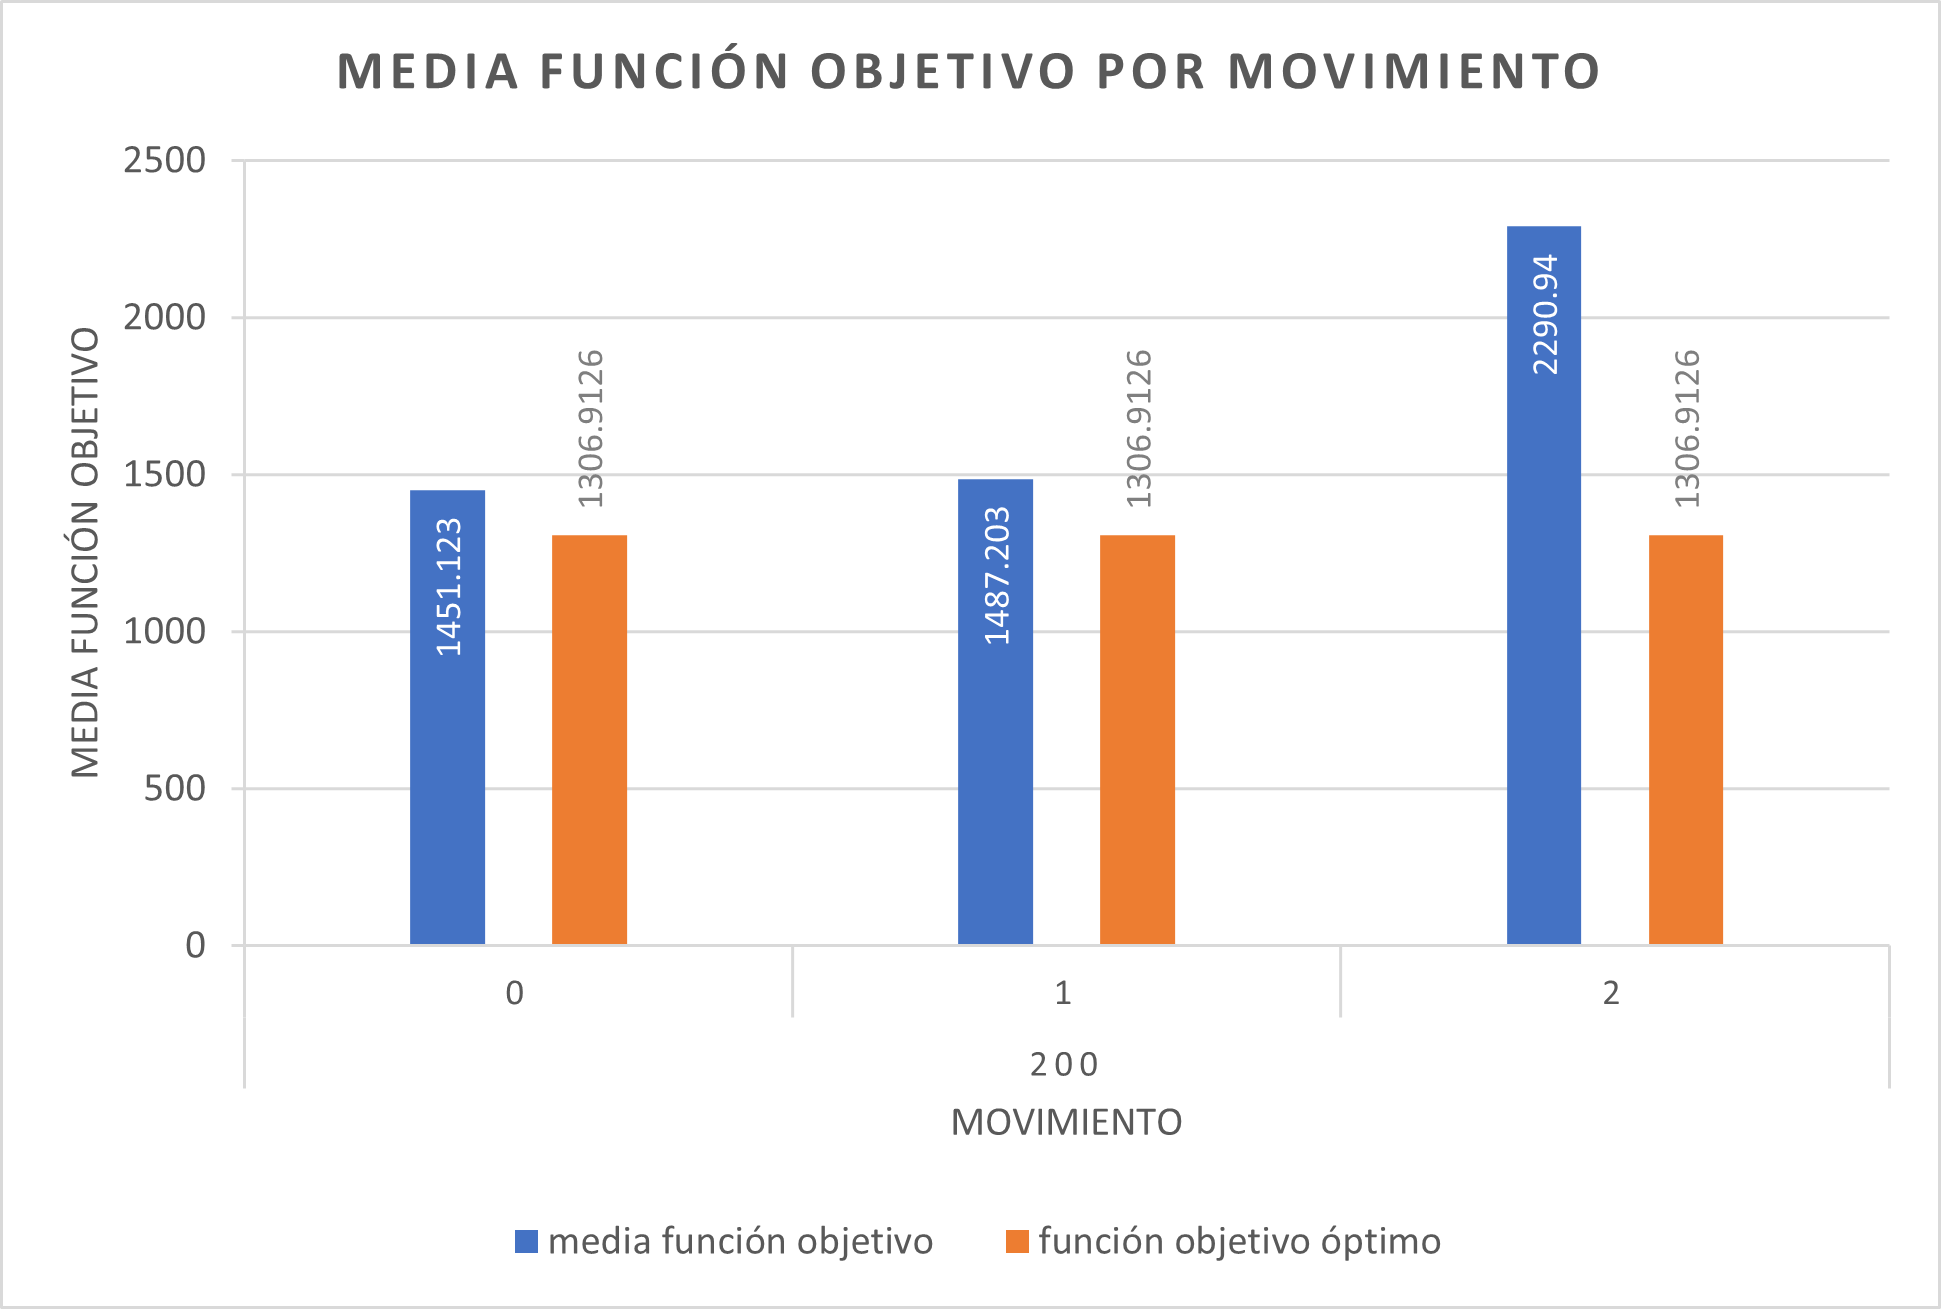
\includegraphics[width=0.8\textwidth]{images/testing/media_por_movimiento_200.png}
    \caption{Media de función objetivo por movimiento para la instancia de dimensión 200.}
    \label{graph:movements_200}
\end{figure}

\subsubsection{Comparación configuraciones}
% - Compare diferencias entre configuraciones distintas de los experimentos.

Para comprar se realizó un gráfico , ver figura \ref{graph:movements}, que muestra los 3 movimientos, de este gráfico se realizó uno similar que muestra solamente los resultados para las instancias $5$ y $200$. 

\begin{figure}[!ht]
    \centering
    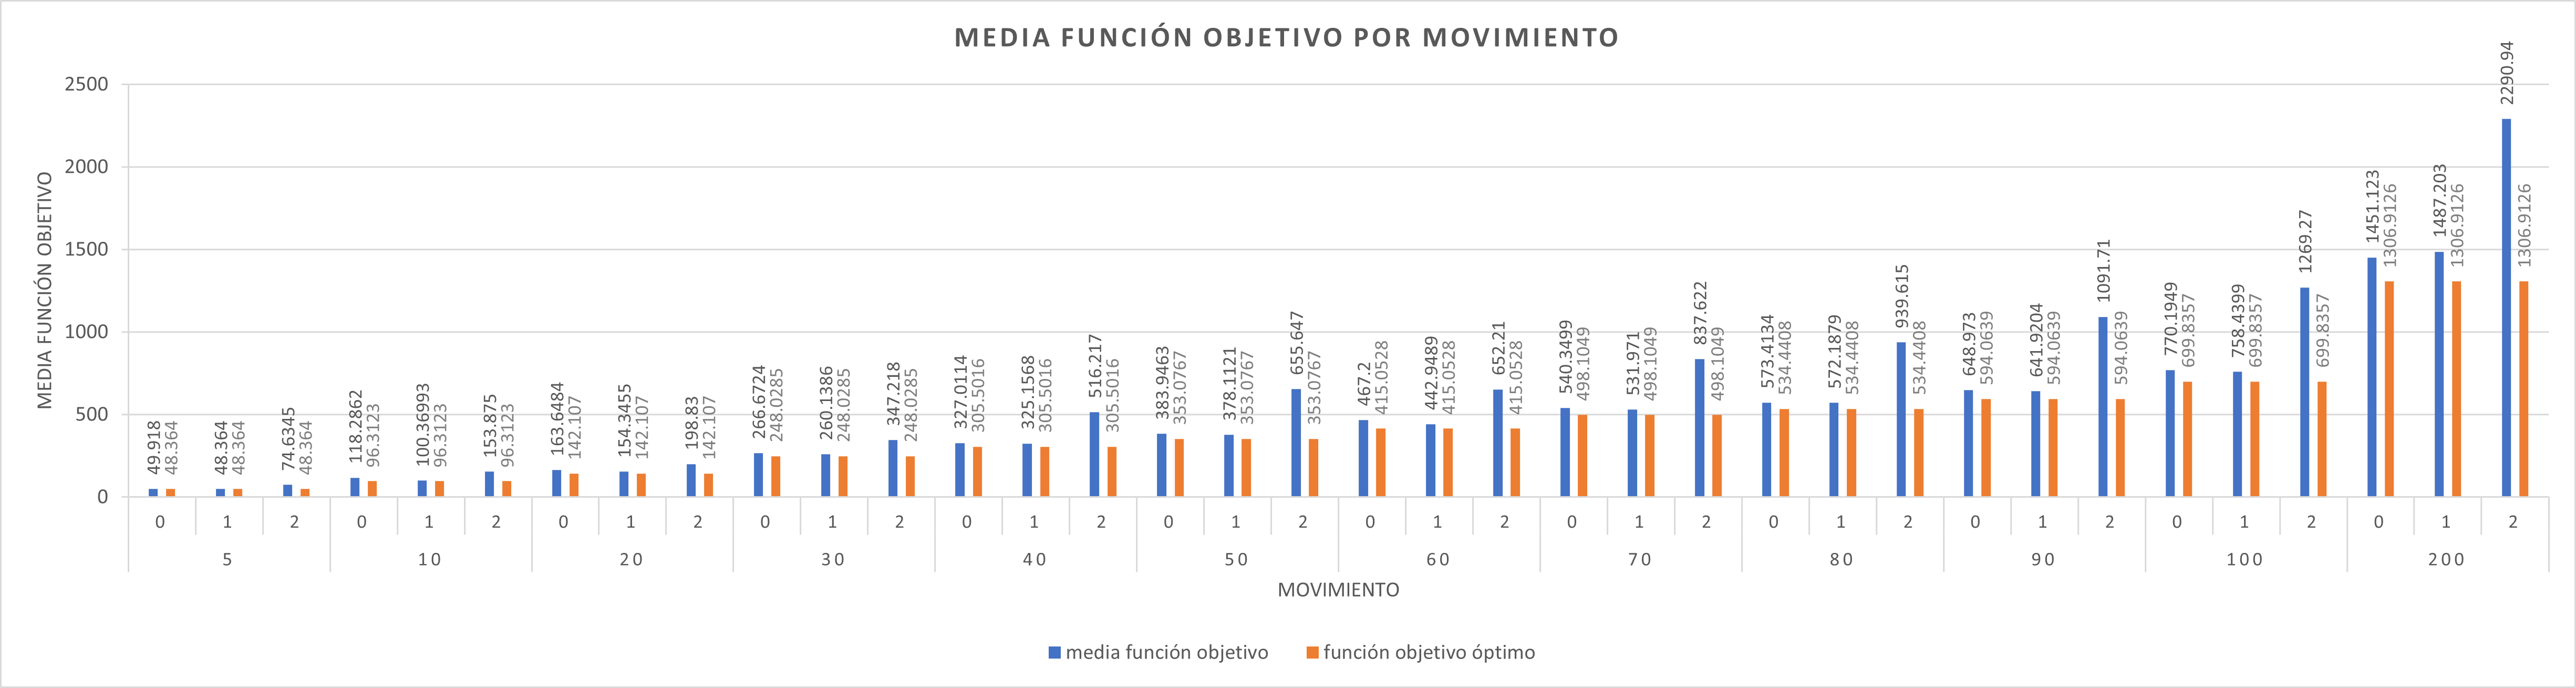
\includegraphics[width=\textwidth]{images/testing/media_por_movimiento.png}
    \caption{Media de función objetivo por movimiento.}
    \label{graph:movements}
\end{figure}

\subsubsection{Análisis}

Para esta experimentación resulta difícil mencionar un movimiento que funcione de la forma más óptima posible para todas las instancias, pero se puede concluir que el movimiento 0 funciona de buena forma para instancias grandes como la 200 pero para instancias pequeñas se aleja un poco del óptimo referencial, el \textit{movimiento 1} funciona de buena manera para las instancias pequeñas y para las más grandes se acerca bastante al óptimo referencial, y el \textit{movimiento 2} no se acerca en absoluto de forma óptima al valor referencial del valor de destrucción.

Un punto destacable es el funcionamiento óptimo para una instancia específica del \textit{movimiento 0}, este movimiento solamente funciona mejor que el \textit{movimiento 1} para la instancia 200, esto puede deberse a algún error en la experimentación o alguna injerencia en la dimensión de la instancia.

